\documentclass{article}

% if you need to pass options to natbib, use, e.g.:
%     \PassOptionsToPackage{numbers, compress}{natbib}
% before loading neurips_2019

% ready for submission
% \usepackage{neurips_2019}

% to compile a preprint version, e.g., for submission to arXiv, add add the
% [preprint] option:
    % \usepackage[preprint]{neurips_2019}

% to compile a camera-ready version, add the [final] option, e.g.:
     \usepackage[final]{style}

% to avoid loading the natbib package, add option nonatbib:
%     \usepackage[nonatbib]{neurips_2019}

\usepackage[utf8]{inputenc} % allow utf-8 input
\usepackage[T1]{fontenc}    % use 8-bit T1 fonts
\usepackage{hyperref}       % hyperlinks
\usepackage{url}            % simple URL typesetting
\usepackage{booktabs}       % professional-quality tables
\usepackage{amsfonts}       % blackboard math symbols
\usepackage{xcolor}         % color text
\usepackage{amsmath}        % for align* environment
\usepackage{nicefrac}       % compact symbols for 1/2, etc.
\usepackage{microtype}      % microtypography
\usepackage{booktabs}
\usepackage{graphicx}       % figures (MoE)

\title{Human Detection in Cross-Environments for Drone-Based Search and Rescue}

% The \author macro works with any number of authors. There are two commands
% used to separate the names and addresses of multiple authors: \And and \AND.
%
% Using \And between authors leaves it to LaTeX to determine where to break the
% lines. Using \AND forces a line break at that point. So, if LaTeX puts 3 of 4
% authors names on the first line, and the last on the second line, try using
% \AND instead of \And before the third author name.

\author{%
  Mahati Manda \\
  Electrical and Computer Engineering \\
  \texttt{mmanda@andrew.cmu.edu} \\
  \And
  Harmony Lau \\
  Electrical and Computer Engineering \\
  \texttt{harmonyl@andrew.cmu.edu} \\
  \And
  Riva Sun \\
  Electrical and Computer Engineering \\
  \texttt{jiaweis2@andrew.cmu.edu} \\
  \AND
  Aditya Singh \\
  Mechanical Engineering \\
  \texttt{as6@andrew.cmu.edu} \\
  \And
  Manasvi Alam \\
  Electrical and Computer Engineering \\
  \texttt{manasvia@andrew.cmu.edu} \\
}

\begin{document}

\maketitle

\section{Introduction}
Please clearly specify the problem you want to solve. In the mid-term report, we expect you to present your baseline methods. Your midterm report should be 4 to 5 pages, excluding reference.

Unmanned aerial vehicles (UAVs) can rapidly survey large, hazardous or inaccessible areas, which has made them central to search-and-rescue (SAR) operations. As coverage scales, however, the bottleneck shifts to human operators, who cannot reliably review the resulting volume of imagery~[1]. Drones must therefore detect people autonomously and reliably across the wide range of environments where people go missing. This is difficult because at high altitudes, a person occupies only a handful of pixels, and against a cluttered background that changes drastically from one terrain to the next.
 
Ciccone and Ceruti address this in [1]. However, their detector is specialized to a single terrain (vegetated wilderness), while real missions also take place over open water and in dense urban areas. The authors themselves report a bias toward vegetated regions that could cause false positives. In our project proposal we therefore asked: \emph{how well can a drone-based human-detection model generalize across distinct physical terrains (maritime, vegetative, and urban) and how much can we improve that generalizability by training across all three terrains rather than any one alone?}
 
This mid-term report covers progress on three methods. We reproduce the baseline of~[1] and match or exceed its reported accuracy (Section~4.1). We build a class-harmonized, domain-balanced multi-domain dataset and fine-tuning pipeline, and design and evaluate a terrain-gated mixture of experts (Sections~3.5 and~4.3).

\section{Related Work}
Please briefly explain the prior work and describe your understanding of their method and how they approached your problem statement. List the relevant previous works that you used/adapted to your project.

\paragraph{Reference method.} Ciccone and Ceruti~[1] adapt YOLO for real-time person detection on a UAV-mounted Jetson Nano. They choose YOLOv5s over newer YOLO versions because of its maturity, well-documented code base, ease of embedded deployment, and because in their preliminary experiments YOLOv8 gave comparable accuracy at higher computational cost. Because Heridal is small, they use two-stage transfer learning approach: pre-training on VisDrone, a large drone dataset rich in small objects, followed by fine-tuning on Heridal. Pre-training on VisDrone improved mAP@50 from 0.665 (Heridal only) to 0.738. Adding the Stanford Drone Dataset as an intermediate stage helps less, and combining all three sources performs worse, which the authors attribute to domain drift. Their Table 3 baseline, unmodified YOLOv5s with the default PANet neck, is the configuration we reproduce for this report.
 
\paragraph{Architectural ablations.} Starting from this baseline, the authors replaced the PANet neck with various feature fusion necks and classification heads. The best YOLOv5 variant, YOLOv5s-PBFPN-Deconv, reaches 0.802 mAP@50 / 0.388 mAP@50:95. They also ported this to YOLOv8s, where PB-FPN gives the best overall accuracy (0.807 / 0.421) but roughly 2.5 times the computation.
 
\paragraph{Findings relevant to our research.} First, the authors found that detection accuracy improved with flight altitude in their field tests, which they explain by the match with Heridal's 40--65\,m capture altitude. The model, fine-tuned on data taken at those specific altitudes, thus performs better (quantify better) for those scenarios. Second, EigenCAM visualizations showed strong activation on vegetation even where no person was present, suggesting the model learned a spurious ``vegetation implies person'' cue from Heridal's forested scenes. Both observations suggest that a single-terrain detector, with images taken at a narrow range of altitudes, may transfer poorly to other environments, which is exactly the gap our project addresses.


\section{Methods}
Explain your understanding of the problem statement. Then focus on the methods that you have done experiments on, and \textbf{clearly explain how your method works. Analyze how your method performs compared to baseline methods. You are encouraged to use formulas and figures to showcase your method.}

To answer our research question, we compare three models:
\begin{enumerate}
    \item[(a)] \textbf{Baseline reproduction:} Yolov5 pre-trained on VisDrone, followed by Heridal fine-tuning, reproducing~[1]. This validates our pipeline against published numbers and serves as the single-terrain reference model for comparison against the rest.
    \item[(b)] \textbf{Multi-domain fine-tuning} (Direction~1 of our proposal): the same VisDrone pre-trained model, but fine-tuned on a domain-balanced combination of Heridal (vegetation), SeaDronesSee~[5] (maritime) and NITC Person Rescue \todo{citation} (urban) dataset.
    \item[(c)] \textbf{Mixture of experts} (Direction~2 of our proposal): three terrain-specific expert detectors and a lightweight CNN gate that routes each image to the matching expert, following Pavlitska et al.~[7].
\end{enumerate}

\subsection{Problem formulation and metrics}
All models solve single-class object detection: given an aerial image, predict bounding boxes and confidence scores for every person. A prediction counts as a true positive (TP) if its intersection-over-union (IoU) with an unmatched ground-truth box reaches a threshold $\tau$, otherwise it is a false positive (FP). Unmatched ground-truth boxes are false negatives (FN). We report
\begin{equation}
    P = \frac{TP}{TP+FP}, \qquad R = \frac{TP}{TP+FN}, \qquad
    \mathrm{AP}_\tau = \int_0^1 P_\tau(R)\,dR,
\end{equation}
where $\mathrm{AP}_\tau$ is the area under the precision--recall curve obtained by sweeping the confidence threshold. With one class, mAP equals AP. We report mAP@50 ($\tau=0.5$) and mAP@50:95, the mean of $\mathrm{AP}_\tau$ over $\tau \in \{0.50, 0.55, \dots, 0.95\}$, which additionally rewards tight localization. Following YOLOv5, $P$ and $R$ are reported at the confidence threshold that maximizes F1. They therefore describe a single operating point, whereas mAP summarizes the whole curve.
 
\subsection{Tools and compute}
All experiments use the Ultralytics YOLOv5 code base~[2] with PyTorch~2.5.1 and CUDA~12.4 under Python~3.11. Training runs on an AWS EC2 \texttt{g4dn.xlarge} instance using the AWS Deep Learning AMI.
 
\subsection{Baseline reproduction}
\label{sec:repro}

\paragraph{Scope of our reproduction.} Given our available compute and time, we reproduce only the Table~3 baseline of~[1], which is unmodified YOLOv5s, rather than the architectural variants. This is because our first priority is the data side of the problem, making the detector work across terrains by changing what it is fine-tuned on. After the mid-term we plan to transfer the most effective architectural changes reported in~[1] (PB-FPN, a P2 head, deconvolution) to our multi-domain models and measure whether their gains carry over across domains.
 
\paragraph{Model.} We use the default YOLOv5s architecture: a CSPDarknet53 backbone, SPPF, a PANet neck and three anchor-based detection heads at P3--P5, with the classification output set to one class. The resulting model has 7.01M parameters and 15.8 GFLOPs at $640\times640$, matching the 7.013M parameters and 15.8 GFLOPs reported in~[1].
 
\paragraph{Stage 1: VisDrone pre-training.} We use VisDrone2019-DET with its official splits (6,471 train / 548 val / 1,610 test-dev). VisDrone has two person-like categories, \emph{pedestrian} and \emph{people}. The paper says only that the ``person'' class was used, so we merge both into a single \emph{person} class and discard all others. Images that then contain no persons are kept as background (negative) images. Training starts from COCO-pretrained \texttt{yolov5s.pt} weights, since the paper does not state its initialization.
 
\paragraph{Stage 2: Heridal fine-tuning.} We obtained Heridal as a Roboflow export with all preprocessing and augmentation disabled (Roboflow's default resize would stretch the 4:3 images to a square, distorting aspect ratio). Image resizing is left to YOLOv5's aspect-preserving letterbox at 640\,px. Following~[1], we pool all images and re-split them randomly 70/20/10 into train/val/test with a fixed seed (seed 0), giving 1,105 / \todo{n} / \todo{n} images. Fine-tuning starts from the stage-1 checkpoint with the highest validation fitness.
 
\paragraph{Training configuration.} We follow the hyperparameter table of~[1] (their Table~1), which matches YOLOv5's built-in \texttt{hyp.scratch-high.yaml} value for value. Both stages use the settings in Table~\ref{tab:hyp}. Augmentation is applied on the fly during training rather than by enlarging the stored dataset. AutoAnchor re-estimates the anchor boxes for each dataset with $k$-means and genetic refinement, as described in~[1]. Early stopping ends a run after 50 epochs without improvement in YOLOv5's fitness score ($0.1\cdot$mAP@50 $+\ 0.9\cdot$mAP@50:95), and the checkpoint with the best fitness is kept.

\begin{table}[h]
  \caption{Hyperparameters, following Table~1 of~[1]. $^\dagger$Set as in~[1], but inactive: copy-paste requires segmentation masks and our labels are boxes only.}
  \label{tab:hyp}
  \centering
  \small
  \begin{tabular}{ll@{\hspace{1.2em}}ll@{\hspace{1.2em}}ll}
    \toprule
    \multicolumn{2}{c}{\emph{Optimizer}} & \multicolumn{2}{c}{\emph{Image augmentation}} & \multicolumn{2}{c}{\emph{Training strategy}} \\
    \cmidrule(r){1-2} \cmidrule(lr){3-4} \cmidrule(l){5-6}
    Optimizer & SGD & \texttt{hsv\_h} & 0.015 & Max epochs & 400 \\
    \texttt{lr0} & 0.01 & \texttt{hsv\_s} & 0.7 & Batch size & 32 \\
    \texttt{lrf} & 0.1 & \texttt{hsv\_v} & 0.4 & Early-stop patience & 50 \\
    Momentum & 0.937 & \texttt{translate} & 0.1 & Image size & $640\times640$ \\
    Weight decay & 0.0005 & \texttt{scale} & 0.9 & AutoAnchor & Enabled \\
     & & \texttt{fliplr} & 0.5 & Split & 70/20/10 \\
     & & \texttt{mosaic} & 1.0 & Seed & Fixed (0) \\
     & & \texttt{mixup} & 0.1 & & \\
     & & \texttt{copy\_paste} & 0.1$^\dagger$ & & \\
    \bottomrule
  \end{tabular}
\end{table}
 
\paragraph{Resolving ambiguities.} Several details needed for an exact reproduction are missing or inconsistent. Table~\ref{tab:ambig} lists the details that~[1] leaves unspecified or states inconsistently, and the choice we made for each. Where the text and Table~1 of~[1] disagree, we follow Table~1.
 
\begin{table}[h]
  \caption{Ambiguities in~[1] and how we resolved them.}
  \label{tab:ambig}
  \centering
  \small
  \begin{tabular}{p{3.2cm}p{4.6cm}p{4.6cm}}
    \toprule
    Item & What~[1] states & Our choice \\
    \midrule
    Reported split & Not stated (val or test) & Report both \\
    Batch size & 16 (text) vs.\ 32 (Table~1) & 32 \\
    Max epochs & 300 (text) vs.\ 400 (Table~1) & 400 \\
    Scale augmentation & $\pm$10\% (text) vs.\ 0.9 (Table~1) & 0.9 \\
    LR scheduler & ``OneCycleLR'' & YOLOv5 cosine one-cycle (\texttt{--cos-lr}) \\
    Initial weights & Not stated & COCO-pretrained YOLOv5s \\
    VisDrone ``person'' & Not defined & \emph{pedestrian} + \emph{people} merged \\
    Heridal split & 70/20/10, method and seed not stated & Random image-level split, seed 0 \\
    \bottomrule
  \end{tabular}
\end{table}
 
\paragraph{Re-splitting Heridal.} The daatset split shipped with the Roboflow export does not follow the protocol of~[1]. Its train and validation sets share the same flights, while its test set consists entirely of flights absent from both. Since~[1] reports a random 70/20/10 split, we re-split the data with a short script to make the results comparable. The script pools every image and its label file from the three original folders, sorts the pooled list by file path, so the starting order is deterministic, shuffles it with a fixed-seed random generator (seed 0), and then assigns the first 70\% of the shuffled images to train, the next 20\% to validation and the remaining 10\% to test. Because the shuffle operates on individual images rather than flights, frames from every location appear in all three splits, making it closer to the reference paper's random Heridal split.
 
\subsection{Multi-Domain Fine-Tuning}
 
\paragraph{Datasets and Label Harmonization.} We combine Heridal (wilderness and vegetation), SeaDronesSee (maritime) and NITC Person Rescue (urban). All annotations are converted to YOLO format and mapped to a single \emph{person} class: in SeaDronesSee, human categories \todo{list exact classes, e.g.\ swimmer} map to \emph{person} and non-human categories (boats, buoys, etc.) are discarded; for NITC, \todo{class mapping}. Merging classes produced a few duplicate boxes on the same person, which YOLOv5 removes automatically. The Heridal portion uses exactly the same train/val/test split as the baseline, so Heridal results are directly comparable across models.
 
\paragraph{Domain Imbalance Issue} The raw training pool is heavily imbalanced: about 75\% of images are maritime. Trained on this pool, the model would mostly learn to detect people in water. Any change in Heridal performance would then be confounded with under-exposure rather than reflecting a genuine multi-domain effect. 
We therefore decide to try different ways of balancing the dataset. Here, we implemented downsampling method and reweighting method.

\begin{table}[h]
    \centering
    \caption{Comparison of downsampling and domain-weighted sampling strategies.}
    \label{tab:comparison}
    \begin{tabular}{lll}
        \toprule
        Aspect & Downsampling & Weighted Sampling \\
        \midrule
        Main approach & Select fewer SeaDronesSee images & Adjust sampling frequency \\
        Dataset size & Reduced training pool & Full training pool retained \\
        Data diversity & Some examples excluded & All examples remain eligible \\
        Small datasets & Unchanged & Sampled more frequently \\
        Repeated images & Not inherently required & Sampling with replacement \\
        Training computation & Usually lower per epoch & Similar to original dataset \\
        Main limitation & Loss of useful examples & Potential overfitting \\
        \bottomrule
    \end{tabular}
\end{table}

The reasons we perform databalancing are as follow:
\begin{itemize}
    \item \textbf{Reduce domain dominance:} SeaDronesSee no longer contributes most of the training images, allowing the model to learn more evenly across environments.
    \item \textbf{Improve cross-domain generalization:} The model receives more balanced exposure to wilderness, maritime, and NITC examples.
    \item \textbf{Reduce training computation:} Fewer images typically mean fewer batches per epoch and faster training.
    \item \textbf{Avoid excessive repetition:} Unlike weighted sampling, downsampling does not require repeatedly selecting images from the smaller datasets.\\
\end{itemize}

\paragraph{Training.} The multi-domain model is initialized from the \emph{same} stage-1 VisDrone checkpoint as the baseline and trained with the identical configuration (Table~\ref{tab:hyp}). The fine-tuning data is therefore the only difference between the two models. AutoAnchor re-estimated anchors for the combined data (best possible recall 0.9998). Notably, about 3.8\% of person boxes (646 of 16,972) are under 3 pixels at the 640\,px training resolution, illustrating how extreme the small-object problem becomes across domains.

\subsubsection{Downsampling}
Downsampling aims to reduce dataset imbalance and prevent the model from being dominated by SeaDronesSee during training. It addresses this imbalance by reducing the number of SeaDronesSee training images while keeping Heridal and NITC unchanged.\\

We downsample SeaDronesSee to the average size of the other two domains (Table~\ref{tab:downsample}). Because SeaDronesSee consists largely of frames extracted from video sequences, we sample deterministically with a fixed stride over the filename-sorted frames (every $k$-th frame, $k=\lfloor 7334/1191 \rfloor = 6$) rather than uniformly at random. This spreads the subsample evenly across all sequences and avoids over-representing individual clips, while discarding mostly redundant near-duplicate frames. The validation set is balanced the same way, so that checkpoint selection is not dominated by one domain either.\\

Suppose we want each dataset to contribute approximately the same number of images. We can set the target number of SeaDronesSee images to the average of Heridal and NITC:
    \begin{align*}
    N_{\text{Sea,target}}=\frac{N_{\text{Heridal}}+N_{\text{NITC}}}{2}
    \end{align*}
    We then randomly select 1,191 images from the original 7,334 SeaDronesSee training images, without replacement. The resulting training distribution becomes:
 
\begin{table}[h]
  \caption{Training images per domain before and after downsampling SeaDronesSee.}
  \label{tab:downsample}
  \centering
  \small
  \begin{tabular}{lrrrr}
    \toprule
    Dataset & Original & Share & After downsampling & Share \\
    \midrule
    Heridal (wilderness) & 1,105 & 11.4\% & 1,105 & 30.7\% \\
    NITC Person Rescue (urban) & 1,277 & 13.1\% & 1,277 & 35.4\% \\
    SeaDronesSee (maritime) & 7,334 & 75.5\% & 1,223 & 33.9\% \\
    \midrule
    Total & 9,716 & & 3,605 & \\
    \bottomrule
  \end{tabular}
\end{table}

However, there is an important limitation: downsampling discards potentially useful training information. Randomly excluded SeaDronesSee images might contain uncommon backgrounds, extremely small swimmers, unusual viewpoints, or challenging lighting conditions. Thus, even though the dataset becomes more balanced, the model may lose important information needed for generalization.\\
 
\subsubsection{Weighted Sampling (not used)}
We use domain-balanced sampling with \(\alpha=0.5\) to reduce the dominance of SeaDronesSee during training (Table~\ref{tab:reweighting}). After reweighting, the expected contribution from Heridal and NITC increases substantially, while SeaDronesSee's contribution decreases from approximately 75\% to 55\%. These percentages represent expected training sampling frequencies, not changes to the actual number of stored images.\\

We assign each image a sampling weight:
\begin{align*}
    w_i=\frac{1}{N_{d(i)}^\alpha}
\end{align*}
where:
\(N_{d(i)}\) is the number of training images in the dataset containing image \(i\), and \(\alpha\) is for balancing strength. With \(\alpha=0.5\), we reduce dataset imbalance without enforcing a completely equal distribution.\\

The model still draws 9,716 images per epoch, with replacement. Thus, smaller datasets are sampled more frequently, and individual images may appear multiple times in an epoch.\\

\begin{table}[h]
  \caption{Training images per domain before and after domain-balanced sampling ($\alpha = 0.5$).}
  \label{tab:reweighting}
  \centering
  \small
  \begin{tabular}{lrrr}
    \toprule
    Dataset & Training images & Original share & Reweighted share \\
    \midrule
    Heridal (wilderness) & 1,105 & 11.37\% & 21.50\% \\
    NITC Person Rescue (urban) & 1,277 & 13.14\% & 23.11\% \\
    SeaDronesSee (maritime) & 7,334 & 75.49\% & 55.39\% \\
    \midrule
    Total & 9,716 & 100.00\% & 100.00\% \\
    \bottomrule
  \end{tabular}
\end{table}

\subsection{Mixture of Experts}

\label{sec:moe}
Our second approach uses a terrain-gated Mixture of Experts (MoE), inspired by Pavlitska et al.~[7]. Instead of training one detector across all terrains, we use three specialized YOLOv5s detectors. A lightweight CNN gating network selects the appropriate expert for each input image (Figure~\ref{fig:moe_arch}).

\begin{figure}[h]
  \centering
  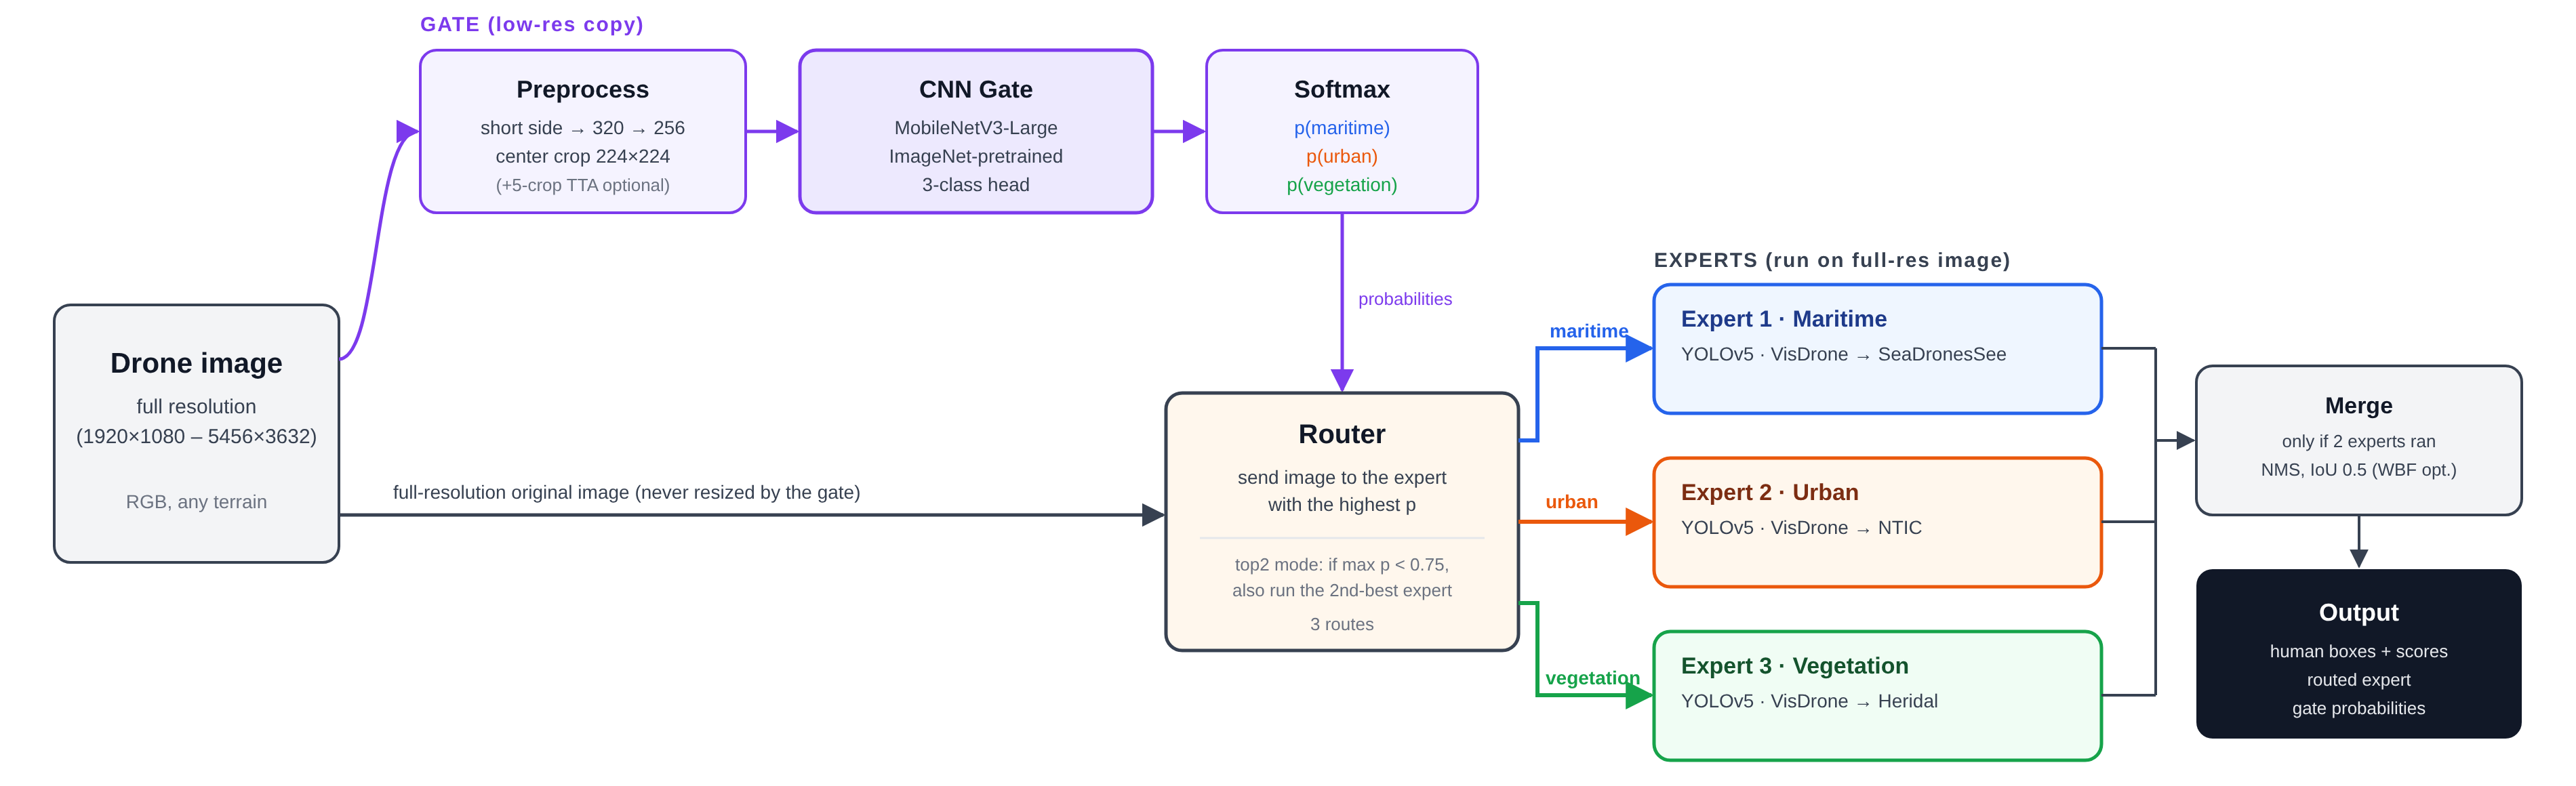
\includegraphics[width=\linewidth]{figures/moe_architecture.png}
  \caption{Terrain-gated mixture of experts. The gate classifies a $224\times224$ copy of the image into maritime, urban or vegetation; the router sends the original full-resolution image to the matching YOLOv5s expert. In the optional top-2 mode, a second expert also runs when the gate is uncertain and the two sets of boxes are merged with NMS.}
  \label{fig:moe_arch}
\end{figure}

\textbf{Terrain-Specific Experts.}
Each expert is initialized from the same VisDrone-pretrained YOLOv5s checkpoint and fine-tuned with the configuration of Table~\ref{tab:hyp} at $640\times640$. The maritime expert is fine-tuned on SeaDronesSee. The urban expert is fine-tuned on NITC Person Rescue. The vegetation expert is fine-tuned on Heridal, so it follows the same recipe as the baseline. All three experts perform single-class human detection.

\textbf{Gating Network.}
We use an ImageNet-pretrained MobileNetV3-Large with a three-class classification head (4.21M parameters, 0.47 GFLOPs, about 3\% of one expert's 15.8 GFLOPs). The gate processes a downsampled, center-cropped image of size $224 \times 224$: the image is resized so its short side is 256 pixels and the center is cropped. We deliberately avoid letterbox padding, because Heridal is the only 4:3 source and padding bars would reveal the dataset rather than the terrain. The selected YOLOv5s expert receives the original image and applies its own preprocessing.

The gate produces three terrain probabilities using softmax:

\begin{equation}
p_d(x) = \frac{\exp(z_d(x))}
{\sum_{j=1}^{3}\exp(z_j(x))}
\end{equation}

Here, $z_d(x)$ is the predicted logit for terrain $d$.

\textbf{Expert Routing.}
We use hard routing to select the expert with the highest terrain probability:

\begin{equation}
d^* = \arg\max_d p_d(x)
\end{equation}

We also include an optional top-2 routing strategy. If the highest probability is below $0.75$, the two most likely experts are executed. Their detections are merged using non-maximum suppression (NMS) with an IoU threshold of $0.5$. Weighted Box Fusion (WBF) is another possible fusion strategy.

\textbf{Gating Network Training.}
We train the gate using terrain labels derived from the source datasets: 8,930 SeaDronesSee images (maritime), 1,277 NITC images (urban) and 1,106 Heridal images (vegetation). Because NITC contains only seven video clips, an early gate learned a narrow notion of ``urban'': it routed only 61.5\% of VisDrone validation images to the urban expert, sending wide grey intersections to maritime and tree-lined streets to vegetation. We therefore add the 6,471 VisDrone2019-DET training images to the urban class, for the gate only; the urban expert is still trained on NITC alone. Inverse-frequency weighted sampling reduces class imbalance. Data augmentation (random resized crops, flips, colour jitter, random JPEG compression, random down-and-up sampling and slight blur) improves robustness to changes in lighting, viewpoint, and image resolution, and discourages the gate from relying on dataset-specific cues such as sharpness or compression. We use AdamW (learning rate $3\times10^{-4}$, weight decay 0.01, batch 32) with cosine learning-rate scheduling and early stopping based on validation macro-F1.

\textbf{Gating Network Results.}
On its own held-out split, the gate achieves $99.85\%$ test accuracy ($1294/1296$). The per-class F1 scores are $1.000$ for maritime, $0.997$ for urban, and $0.994$ for vegetation; both errors are a Heridal scene with houses and a road, classified as urban. All 548 VisDrone validation images, which the gate did not see during training, are routed to the urban expert. However, these results measure terrain classification rather than human detection. The test splits are also largely in-domain.

\textbf{Evaluation.}
The MoE is evaluated on the same per-domain test sets as the other models (Section~\ref{sec:moe_results}). Because the full pipeline (gate, router and expert) is not a single YOLOv5 model, we score it with our own evaluation script that follows YOLOv5's \texttt{val.py}: confidence threshold 0.001, NMS IoU 0.6, the same greedy matching over IoU thresholds 0.50--0.95, 101-point interpolated AP, and $P$ and $R$ at the maximum-F1 confidence. As a consistency check, the vegetation expert scored by our script on SeaDronesSee gives 0.196 mAP@50 / 0.064 mAP@50:95, close to the \texttt{val.py} result of the baseline (0.187 / 0.064), which uses the same training recipe. We also report routing accuracy, a routing ablation and inference cost.


\section{Results}
Please report your result in this section. Analyze your result with your evaluation metrics. Show visual results if possible, and be sure to show the results of you baseline methods.

\paragraph{Evaluation protocol.} All models are evaluated with YOLOv5's \texttt{val.py} at $640\times640$, with a confidence threshold of 0.001 and an NMS IoU threshold of 0.6. To expose cross-domain trade-offs, each model is evaluated separately on the test set of each domain rather than only on a pooled test set.

\subsection{Baseline Reproduction Results}

Table~\ref{tab:baseline} compares our reproduced baseline with Table~3 of~[1]. Our model matches the paper's parameter count and computation and exceeds its reported accuracy on both of our splits: by 9.9 / 6.9 points mAP@50 and 10.5 / 7.2 points mAP@50:95 on validation / test, respectively. The validation-to-test gap of about 3 points is modest, indicating that the model selected by validation fitness does not overfit the validation set.
 
\begin{table}[h]
  \caption{Baseline (YOLOv5s, VisDrone $\rightarrow$ Heridal) compared with Table~3 of~[1]. Differences are shown in parentheses.}
  \label{tab:baseline}
  \centering
  \small
  \begin{tabular}{lccc}
    \toprule
    Metric & Paper~[1] & Ours (val) & Ours (test) \\
    \midrule
    mAP@50 & 0.738 & 0.837 (+0.099) & 0.807 (+0.069) \\
    mAP@50:95 & 0.343 & 0.448 (+0.105) & 0.415 (+0.072) \\
    Precision & 0.799 & 0.850 (+0.051) & 0.826 (+0.027) \\
    Recall & 0.670 & 0.771 (+0.101) & 0.740 (+0.070) \\
    \midrule
    Parameters / GFLOPs & 7.013M / 15.8 & \multicolumn{2}{c}{7.01M / 15.8} \\
    \bottomrule
  \end{tabular}
\end{table}
 
We consider the reproduction successful, since the published pipeline reaches at least the reported accuracy. Several factors plausibly explain why we exceed it:
\begin{itemize}
    \item \textbf{Dataset version and split.} We used a Roboflow export of Heridal and our own random 70/20/10 split. Since we may have used a different version of the Heridal dataset, different annotation tightness  would have affected the mAP@50:95 in particular, and the composition of a small test set ($\approx$160 images) can shift mAP by several points.
    \item \textbf{Configuration choices.} Where~[1] is internally inconsistent we followed its Table~1 (batch 32, up to 400 epochs), which may differ from the setting behind its reported numbers.
    \item \textbf{Software versions.} We use a newer YOLOv5 and PyTorch release than the authors, which may differ in loss computation and evaluation details.
\end{itemize}
All results come from a single training run. Quantifying run-to-run variance over several seeds and splits is planned in the future.

\subsection{Multi-Domain Fine-Tuning Results}
\subsubsection{Downsampling}
\begin{table}[h]
  \caption{Baseline (VisDrone $\rightarrow$ Heridal) vs.\ multi-domain fine-tuning (VisDrone $\rightarrow$ Heridal + SeaDronesSee + NITC, downsampled), evaluated separately on each domain's test set. Best value per domain in bold.}
  \label{tab:multidomain}
  \centering
  \small
  \begin{tabular}{llcccc}
    \toprule
    Test set & Model & Precision & Recall & mAP@50 & mAP@50:95 \\
    \midrule
    Heridal (vegetation) & Baseline & 0.826 & 0.740 & 0.807 & \textbf{0.415} \\
    {\footnotesize 159 img, 288 persons} & Multi-domain & \textbf{0.842} & \textbf{0.757} & \textbf{0.828} & 0.404 \\
    \midrule
    SeaDronesSee (maritime) & Baseline & 0.330 & 0.259 & 0.187 & 0.064 \\
    {\footnotesize 1,047 img, 4,372 persons} & Multi-domain & \textbf{0.808} & \textbf{0.762} & \textbf{0.760} & \textbf{0.320} \\
    \midrule
    NITC (urban) & Baseline & 0.109 & 0.040 & 0.024 & 0.005 \\
    {\footnotesize 182 img, 1,367 persons} & Multi-domain & \textbf{0.985} & \textbf{0.990} & \textbf{0.992} & \textbf{0.814} \\
    \midrule
    Mean over domains & Baseline & & & 0.339 & 0.161 \\
     & Multi-domain & & & \textbf{0.860} & \textbf{0.513} \\
    \bottomrule
  \end{tabular}
\end{table}

<TODO> 
Table~\ref{tab:multidomain} compares the single-domain baseline with the multi-domain model on each terrain. The baseline transfers poorly outside its training terrain: on SeaDronesSee its mAP@50 falls to 0.187, and on NITC it fails almost entirely (0.024). A likely contributor is object scale. Heridal's people are tiny, so AutoAnchor fits the baseline's anchors to very small boxes, and~[1] notes that a model trained only on very small objects learns to detect only very small objects. The larger, closer-range people in the urban NITC imagery therefore fall outside what the baseline has learned. Multi-domain fine-tuning removes this failure, raising mAP@50 to 0.760 on SeaDronesSee and 0.992 on NITC, and lifting the mean over domains from 0.339 to 0.860.

Importantly, this broader coverage does not come at the cost of the original terrain. On Heridal the multi-domain model slightly improves precision (0.842 vs.\ 0.826), recall (0.757 vs.\ 0.740) and mAP@50 (0.828 vs.\ 0.807), while mAP@50:95 is marginally lower (0.404 vs.\ 0.415), suggesting slightly looser localization. With a test set of only 159 images, differences of this size (1--2 points) are within the range expected from run-to-run variation, so we conclude that adding maritime and urban data leaves Heridal performance essentially unchanged.

These results should be read as in-domain performance. The multi-domain model has seen all three terrains during training, so its gains on SeaDronesSee and NITC show broader coverage rather than generalization to unseen terrain. The near-perfect NITC score also likely reflects near-duplicate video frames shared between its training and test splits. Evaluating both models on locations absent from all training data remains the decisive test of our research question and is the next step.

Table~\ref{tab:balancing_results_reweighting} compares the single-domain baseline with the multi-domain model trained using domain-balanced weighted sampling $\alpha=0.5$. The baseline transfers poorly to environment outside its Heridal training domain, achieving an mAP@50 only 0.187 on SeaDroneSee and 0.024 on NITC. In contrast, weighted multi-domain fine-tuning improves detection performance across all three environments. On SeaDroneSee, mAP@50 increases from 0.187 to 0.844, and mAP@50:95 goes from 0.064 to 0.408. Similarly, NITC mAP@50 increases to 0.991, with mAP@50:95 reaching 0.806, compared with only 0.024 and 0.005 for the baseline. Overall, the mean mAP@50 across domains increases from 0.339 to \textbf{0.893}, and mean mAP@50:95 improves from 0.161 to \textbf{0.549}.\\

Importantly, these improvements do not come at the expense of the original Heridal domain. Unlike the baseline, which has an mAP@50 of 0.807 and mAP@50:95 of 0.415, the weighted multi-domain model improves both metrics to \textbf{0.843} and \textbf{0.433} respectively. Precision also increases from 0.826 to 0.834, while recall rises from 0.740 to 0.788. These results suggest that multi-domain fine-tuning can improve detection across different environments while preserving, and potentially enhancing, performance on the original search-and-rescue terrain.\\

A potential advantage of weighted sampling is that it addresses dataset imbalance without discarding training examples. Rather than downsampling SeaDronesSee, which originally accounts for 75.49\% of the training images, weighted sampling adjusts the expected training distribution to 21.50\% Heridal, 23.11\% NITC, and 55.39\% SeaDronesSee. This increases exposure to the smaller domains while preserving the full diversity of maritime imagery. The resulting performance improvements are consistent with the hypothesis that maintaining diverse training examples while reducing domain dominance benefits multi-domain person detection. However, these results alone do not establish that weighting is the direct cause of the improvement over the single-domain baseline, since both the training domains and sampling strategy have changed.



\begin{table}[h]
  \caption{Baseline (VisDrone $\rightarrow$ Heridal) vs.\ multi-domain fine-tuning (VisDrone $\rightarrow$ Heridal + SeaDronesSee + NITC, Weighted sampling), evaluated separately on each domain's test set. Best value per domain in bold.}
  \label{tab:balancing_results_reweighting}
  \centering
  \small
  \begin{tabular}{llcccc}
    \toprule
    Test set & Model & Precision & Recall & mAP@50 & mAP@50:95 \\
    \midrule
    Heridal (vegetation) & Baseline & 0.826 & 0.740 & 0.807 & 0.415 \\
    {\footnotesize 159 img, 288 persons} & Multi-domain & \textbf{0.834} & \textbf{0.788} & \textbf{0.843} & \textbf{0.433} \\
    \midrule
    SeaDronesSee (maritime) & Baseline & 0.330 & 0.259 & 0.187 & 0.064 \\
    {\footnotesize 1,047 img, 4,372 persons} & Multi-domain & \textbf{0.876} & \textbf{0.848} & \textbf{0.844} & \textbf{0.408} \\
    \midrule
    NITC (urban) & Baseline & 0.109 & 0.040 & 0.024 & 0.005 \\
    {\footnotesize 182 img, 1,367 persons} & Multi-domain & \textbf{0.980} & \textbf{0.980} & \textbf{0.991} & \textbf{0.806} \\
    \midrule
    Mean over domains & Baseline & & & 0.339 & 0.161 \\
     & Multi-domain & & & \textbf{0.893} & \textbf{0.549} \\
    \bottomrule
  \end{tabular}
\end{table}

\subsection{Mixture of Experts Results}
\label{sec:moe_results}

\paragraph{Routing.} On the shared test sets the gate routes all 1,388 images to the correct expert (1,047/1,047 maritime, 182/182 urban, 159/159 vegetation). Its top probability exceeds 0.75 on every image, so top-2 routing never triggers and top-1 and top-2 give identical results. Every MoE error is therefore a detection error of the chosen expert, not a routing error.

\begin{table}[h]
  \caption{Baseline, both multi-domain models and the mixture of experts, evaluated separately on each domain's test set. Best value per domain in bold.}
  \label{tab:moe}
  \centering
  \small
  \begin{tabular}{llcccc}
    \toprule
    Test set & Model & Precision & Recall & mAP@50 & mAP@50:95 \\
    \midrule
    Heridal (vegetation) & Baseline & 0.826 & 0.740 & 0.807 & 0.415 \\
    {\footnotesize 159 img, 288 persons} & Multi-domain (downsampled) & \textbf{0.842} & 0.757 & 0.828 & 0.404 \\
     & Multi-domain (weighted) & 0.834 & \textbf{0.788} & \textbf{0.843} & \textbf{0.433} \\
     & MoE (ours) & 0.803 & 0.781 & 0.801 & 0.369 \\
    \midrule
    SeaDronesSee (maritime) & Baseline & 0.330 & 0.259 & 0.187 & 0.064 \\
    {\footnotesize 1,047 img, 4,372 persons} & Multi-domain (downsampled) & 0.808 & 0.762 & 0.760 & 0.320 \\
     & Multi-domain (weighted) & \textbf{0.876} & \textbf{0.848} & \textbf{0.844} & \textbf{0.408} \\
     & MoE (ours) & 0.834 & 0.809 & 0.806 & 0.371 \\
    \midrule
    NITC (urban) & Baseline & 0.109 & 0.040 & 0.024 & 0.005 \\
    {\footnotesize 182 img, 1,367 persons} & Multi-domain (downsampled) & \textbf{0.985} & \textbf{0.990} & \textbf{0.992} & \textbf{0.814} \\
     & Multi-domain (weighted) & 0.980 & 0.980 & 0.991 & 0.806 \\
     & MoE (ours) & 0.980 & 0.987 & \textbf{0.992} & 0.800 \\
    \midrule
    Mean over domains & Baseline & & & 0.339 & 0.161 \\
     & Multi-domain (downsampled) & & & 0.860 & 0.513 \\
     & Multi-domain (weighted) & & & \textbf{0.893} & \textbf{0.549} \\
     & MoE (ours) & & & 0.866 & 0.514 \\
    \bottomrule
  \end{tabular}
\end{table}

\paragraph{Comparison with the other models.} Table~\ref{tab:moe} compares the MoE with the baseline and both multi-domain models. Against the single-domain baseline, the MoE raises mean mAP@50 from 0.339 to 0.866 and mean mAP@50:95 from 0.161 to 0.514, because each terrain is now handled by an expert trained on it. Against downsampled multi-domain fine-tuning it is on par on average (0.866 vs.\ 0.860 mAP@50, 0.514 vs.\ 0.513 mAP@50:95), but the per-domain picture differs: the MoE is clearly better on SeaDronesSee (+0.046 mAP@50, +0.051 mAP@50:95), equal on NITC, and worse on Heridal ($-0.027$ / $-0.035$). Multi-domain fine-tuning with weighted sampling, however, outperforms the MoE on SeaDronesSee ($-0.038$ / $-0.037$ for the MoE) and Heridal ($-0.042$ / $-0.064$), matches it on NITC, and has the best mean (0.893 / 0.549).

The Heridal result explains much of this. The vegetation expert follows the same recipe as the baseline and scores almost the same (0.801 vs.\ 0.807 mAP@50), so the MoE inherits single-domain performance on Heridal. The multi-domain models improve Heridal beyond the baseline, which suggests that people seen in the other two terrains help on the smallest dataset. Specialization keeps each expert free of interference from other domains, but it also prevents this transfer. With the full SeaDronesSee pool available through weighted sampling, a single shared model is the stronger choice in our experiments.

\paragraph{Is the gate necessary?} Table~\ref{tab:moe_ablation} isolates the routing. Each expert collapses outside its own terrain (for example, the maritime expert reaches only 0.014 mAP@50 on NITC), so no single expert is usable on its own. Running all three experts on every image and merging their boxes with NMS avoids routing altogether but is clearly worse than the MoE (0.757 vs.\ 0.866 mean mAP@50) at three times the detection compute: off-domain experts add false positives that do not overlap a correct box and therefore survive NMS, which is most damaging on SeaDronesSee (0.576 vs.\ 0.806).

\begin{table}[h]
  \caption{Routing ablation on the shared test sets (mAP@50 / mAP@50:95). ``All 3 + NMS'' runs every expert on every image and merges the boxes.}
  \label{tab:moe_ablation}
  \centering
  \small
  \begin{tabular}{lcccc}
    \toprule
    Method & Heridal & SeaDronesSee & NITC & Mean \\
    \midrule
    Maritime expert only & 0.030 / 0.009 & \textbf{0.806} / \textbf{0.371} & 0.014 / 0.004 & 0.284 / 0.128 \\
    Urban expert only & 0.003 / 0.001 & 0.024 / 0.010 & \textbf{0.992} / \textbf{0.800} & 0.340 / 0.271 \\
    Vegetation expert only & \textbf{0.801} / \textbf{0.369} & 0.196 / 0.064 & 0.006 / 0.002 & 0.334 / 0.145 \\
    All 3 experts + NMS & 0.709 / 0.328 & 0.576 / 0.235 & 0.985 / 0.776 & 0.757 / 0.446 \\
    MoE, gate + top-1 routing & \textbf{0.801} / \textbf{0.369} & \textbf{0.806} / \textbf{0.371} & \textbf{0.992} / \textbf{0.800} & \textbf{0.866} / \textbf{0.514} \\
    \bottomrule
  \end{tabular}
\end{table}

\paragraph{Cost.} Per image, the MoE runs the gate and one expert: about 16.3 GFLOPs, 3\% more than a single YOLOv5s (15.8 GFLOPs). It must, however, store three experts and the gate (25.2M parameters, versus 7.01M for one multi-domain model). On an Apple-silicon laptop GPU (PyTorch MPS), the mean time per image was 84\,ms for the MoE versus 111\,ms for running all three experts; the gate accounts for 47\,ms of this, mostly spent downscaling the 4K input on the CPU, which can be optimized.

\paragraph{Qualitative results.} Figure~\ref{fig:moe_examples} shows MoE predictions on each test set. Many of the remaining ``errors'' are annotation issues rather than detection failures. On SeaDronesSee, several sequences have ground-truth boxes shifted by a few pixels; for swimmers only a few pixels wide this drops the IoU below 0.5, so a correct detection is counted as both a false positive and a false negative. On NITC, some of the false positives are visible people who are not labeled. Genuine failures are concentrated in crowded Heridal scenes, where small, partly occluded people are missed.

\begin{figure}[h]
  \centering
  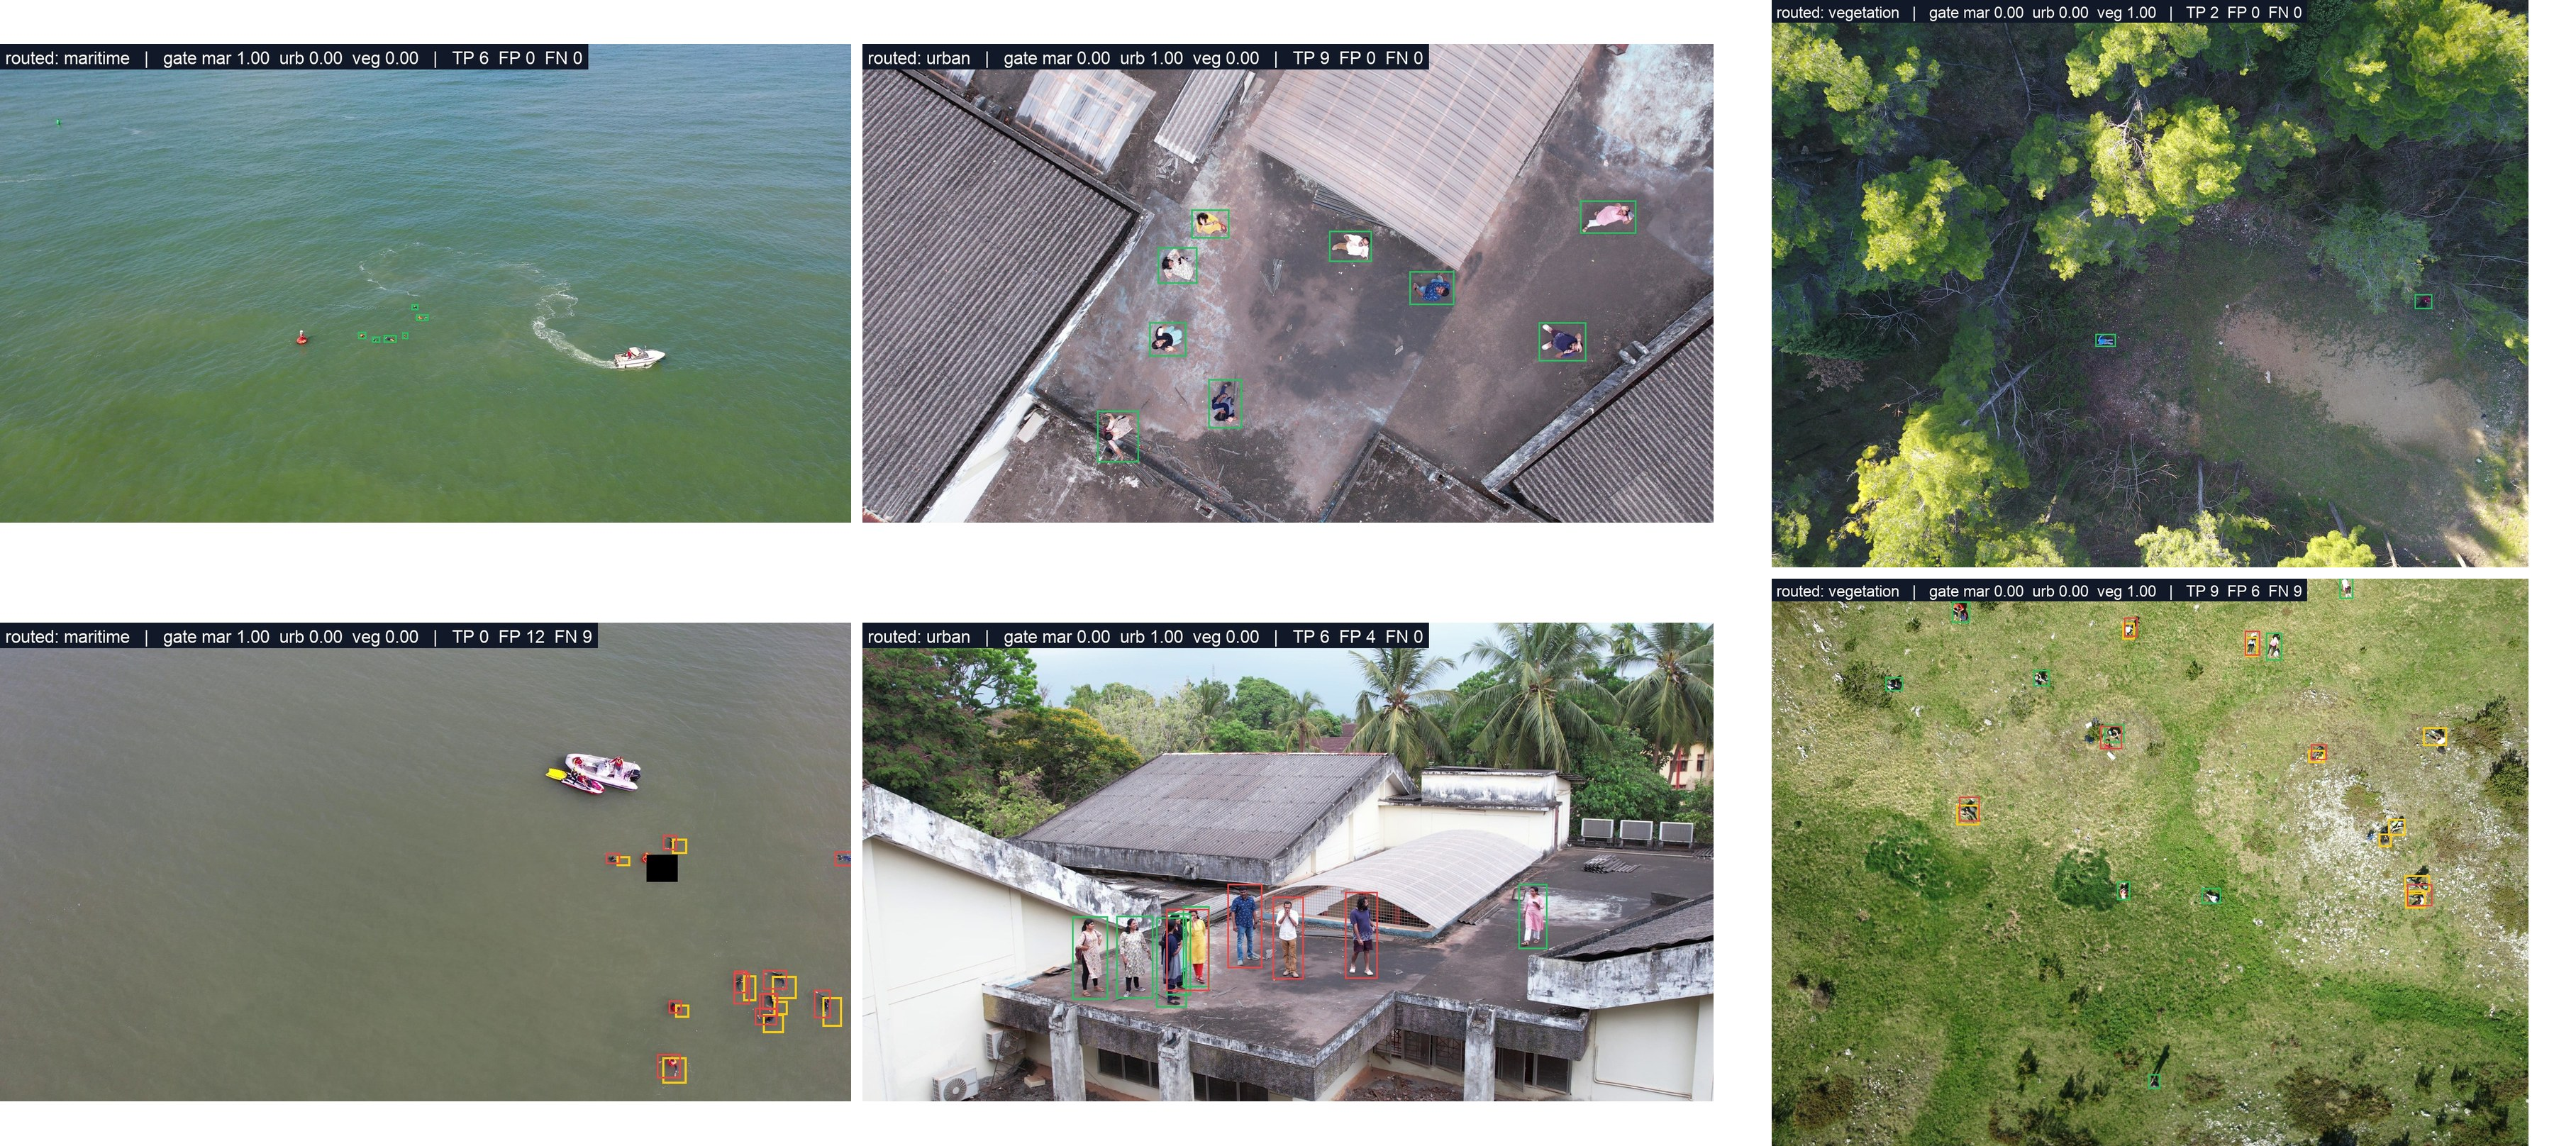
\includegraphics[width=\linewidth]{figures/moe_examples.jpg}
  \caption{MoE detections at confidence $\geq 0.25$ on SeaDronesSee, NITC and Heridal (left to right). Green: correct detection (IoU $\geq 0.5$); red: false positive; yellow: missed person. Top row: typical successes. Bottom row: typical failures, namely ground-truth boxes offset from the swimmers (left), unlabeled people counted as false positives (middle), and missed small people in a crowded vegetated scene (right). The banner shows the routed expert and the gate probabilities.}
  \label{fig:moe_examples}
\end{figure}

\paragraph{Limitations.} All test images come from the same three datasets the experts were trained on, so these are in-domain results. The gate's labels are dataset identities, and the gate was trained on splits that were made before the team's shared re-split, so some test images may have been seen by the gate during training; this can only inflate routing accuracy, not the experts' detection scores, and routing on unseen VisDrone images is equally accurate. All results come from a single training run per model.

\section{Ablation Study (if applicable)}
You may have several ideas and components of your project pipeline you wish to explore; Since some of these components may be more or less important, you should run isolated experiments with them and find how each part is affecting your final result.



\section{Discussion and Conclusion}
What have you found during the project? What conclusion can you draw? Is there any improvement compared to prior work? Are there any limitations? 

<could be because just Heridal fine tuning caused overfitting -- false positives, it's learned to separate "vegetation" from spurious human detection, since the other datasets balanced it out>

<baseline seadronessee and nitc is so bad, it basically isnt able to detect the people at all even though theyre actually very visible in the frames, signalling that the heridal fine tuning has completely removed the ability to detect humans of a normal size, cos it is so used to detecting humans that are like 5 pixels wide against vegetation.>

<the reason for the very high test accuracy is probably because the images included in the different splits are likely consecutive frames from the same flight, since most of the datasets are video frames (cite) from a long video, and the split is randomised. the model may not do so well on a completely unseen flight>

<however, one very nice thing to see is that the multi domain fine-tuned model is able to now detect humans at different altitudes, angles and most importantly across different backgrounds/terrains>

\section*{References}

\small
[1] Ciccone, F. \& Ceruti, A. (2025) Real-Time Search and Rescue with Drones: A Deep Learning Approach for Small-Object Detection Based on YOLO. Drones 9(8):514.

\section{Archive}
\subsubsection{Weighted Sampling}


\end{document}